\documentclass[11pt]{article}
\usepackage[margin=1in]{geometry}
\usepackage{times}
\usepackage{tikz}
\usepackage{pgfplots}
\pgfplotsset{compat=1.18}
\usetikzlibrary{arrows.meta, positioning, shapes.geometric, fit,
                 backgrounds, matrix, calc, decorations.pathreplacing}
\usepackage{booktabs}
\usepackage{amsmath}
\usepackage{graphicx}
\usepackage{hyperref}

\title{AI Metadata and Session Data Repository:\\
       A Client Architecture for Managing, Measuring, and Mitigating\\
       Enterprise Generative AI}

\author{Johnny Morgan \\ UMBC Department of Information Systems \\ \texttt{yj07538@umbc.edu}}

\date{\today}

\begin{document}
\maketitle

\begin{abstract}
Enterprises are deploying generative AI into business processes without the
instrumentation needed to manage it. We propose a client architecture that
captures AI utilization metadata and session data as the precondition for
managing AI systems: an inventory of AI tools and instances, quantitative and
qualitative measures of utilization and effectiveness (KPIs, MOEs, MOPs), and
the capture substrate required to detect, measure, and mitigate hallucinations
as they emerge. We argue that AI failure modes are retrospective and emergent,
so capture must be comprehensive; anything not captured before it emerges is
permanently unavailable to retrospective study. We describe the repository's
reference architecture, its immutable-event data model, a measurement
framework, and a hallucination risk lifecycle modeled on adverse-event
surveillance. We close with a set of dated, falsifiable predictions.
\end{abstract}

% ---------------------------------------------------------------------------
\section{Introduction}

Organizations are placing generative AI into their business processes faster than
they are building the means to manage it. A model now drafts customer replies,
writes code, summarizes documents, and helps make decisions, and each use carries
both a promise and a hazard. The promise is that AI raises what a workforce can
produce. The hazard is that a generative model can be wrong in ways that are
fluent and confident, and a wrong answer can move into a business process and
cause harm. Governance frameworks and regulation have begun to treat the record of
how AI is used as an obligation rather than an option
\cite{nist2023airmf, euaiact2024}. Most deployments keep no such record.

The specific problem is that an uninstrumented AI deployment cannot be managed. An
organization that does not capture how its AI is used cannot measure the return on
what it spends, and it cannot prove the value that would justify the investment. It
also cannot see the failures. The efficacy of a system prompt or a user prompt is
not guaranteed, and a prompt that works today can induce a hallucination under a
different input, a longer context, or a changed model. Without a record that
hallucination passes undetected and unmitigated, and the harm can propagate and
cascade into corporate embarrassment and liability. Value and risk are invisible
for the same reason: there is nothing to look at.

In this paper we propose a client architecture that captures AI utilization
metadata and session data as the precondition for managing AI in an organization.
The architecture is simple at the top and its complexity is a drill-down. The AI
systems in use are instrumented, their session content is stored, metadata is
derived into a small set of repositories separated by sensitivity, and outcomes
and risks are drawn from that metadata and reported to the organization. We argue
that capture has to come before the questions it will answer, because the
behaviors worth measuring, from a new failure mode to a new objective, are not
known when the data is captured, and anything not captured before it emerges is
lost to later study. On this record the harms of AI become foreseeable,
detectable, and mitigatable, and the value of AI, including how far it multiplies
human capital, becomes calculable. This is a proposal and a theory of operation,
not a report of results.

This differs from the tools that instrument AI today. Current operational tooling
is largely monitoring: it traces calls and scores them against evaluations chosen
in advance, and it serves developers building a single application
\cite{majors2022observability}. Monitoring answers questions its designers already
hold. The failures and the value that matter most to an organization are the ones
nobody thought to declare, so an enterprise needs an observability substrate rather
than a monitoring dashboard, and it needs that substrate to carry governance and
continuity as well as measurement. We treat hallucination detection, which a body
of work addresses on its own \cite{ji2023hallucination}, as one risk detector
within this larger system rather than as the system itself.

The remainder of the paper is organized as follows.
Section~\ref{sec:problem} sets out the management problem and the use cases that
make the record indispensable. Section~\ref{sec:epistemology} gives the
epistemological argument for capturing before questioning.
Section~\ref{sec:related} positions the work against observability tooling and
governance frameworks. Section~\ref{sec:architecture} describes the architecture
and Section~\ref{sec:datamodel} its data model. Section~\ref{sec:measurement}
develops measurement, portfolio reporting, and the outcome repository.
Section~\ref{sec:risk} treats outcomes and the hallucination taxonomy, and
Sections~\ref{sec:obligations} and~\ref{sec:trust} treat the obligations AI must
meet and the trust it must earn. Section~\ref{sec:operation} describes operation
and the planned
continuity capability. Section~\ref{sec:predictions} states the paper's
predictions, Section~\ref{sec:governance} its governance, and
Section~\ref{sec:limits} its limits.

% ---------------------------------------------------------------------------
\section{The Problem: Managing AI Without Visibility}
\label{sec:problem}

Organizations are placing generative AI into everyday business processes faster
than they are building the means to see what it does. A model drafts a contract
clause, answers a customer, writes code, or summarizes a case file, and the
interaction leaves little behind. The output is used and the conditions that
produced it are gone. An organization in this position runs a process it cannot
inspect.

The gap is not a single missing dashboard. It is a set of questions an
organization cannot answer about its own use of AI. A manager accountable for a
deployment would want to establish each of the following and today usually
cannot.

\paragraph{Inventory.} Which AI tools, models, and instances are in use, by whom,
and at what version. Adoption often runs ahead of any record of it, so the
inventory itself is unknown.

\paragraph{Utilization and cost.} How much the organization uses AI, measured in
sessions, tokens, and spend, and how that use is distributed across teams and
workflows.

\paragraph{Effectiveness.} Whether the AI is doing useful work. Task success,
rework, acceptance, and escalation are the measures of performance and
effectiveness that would tell a manager whether the deployment earns its cost.

\paragraph{Risk.} How often the model produces wrong or fabricated output,
whether such failures recur, and whether they cascade into downstream work.
Hallucination incidence, and its trajectory over time, are invisible without a
record of the interactions that carried them.

\paragraph{Degradation within a session.} How context-window utilization and
context rot affect output quality as a session lengthens, and when a session has
grown long enough that its output can no longer be trusted.

\paragraph{The people and the model.} How skillfully the workforce uses the
tools, and how the model's own behavior shifts over time.

The natural response is to add metrics. That response fails for the reason
developed in Section~\ref{sec:epistemology}: the failures that matter are not
known in advance, so a fixed set of metrics measures the wrong things. What the
organization lacks is not a dashboard but a record. The rest of this paper
describes that record and the architecture around it.

\subsection{Why the record is indispensable}

An organization that puts a generative model into a business process takes on a
risk it cannot see without a record. The efficacy of a system prompt or a user
prompt is not a given. The same prompt that works today can, under a different
input, a longer context, or a changed model, induce a hallucination. That
hallucination can pass into the business process undetected, because nothing in an
uninstrumented deployment is watching for it, and unmitigated, because nothing
catches it. From there the harm can propagate into downstream work and cascade
across a chain of decisions, and at the end of that chain are corporate
embarrassment and corporate liability.

What makes the absence of the record indefensible is that these events are
foreseeable, detectable, and mitigatable. They are foreseeable because prompt
efficacy is known not to be guaranteed. They are detectable because the
interaction that carried the fault can be examined. They are mitigatable because a
detected fault can be corrected before it spreads. An organization that could have
foreseen, detected, and mitigated a harm, and did not because it kept no record,
owns the consequence. The architecture is what turns a foreseeable, detectable,
and mitigatable harm from a realized loss into a managed one. Three cases show the
difference.

\paragraph{A prompt that quietly stops working.} A system prompt constrains a
customer-facing assistant until a customer's phrasing pushes the model outside it,
and the assistant states a policy the company does not hold. Without the record no
one knows until a customer acts on it. With the record the interaction is
captured, the deviation from the system prompt is detected, and the pattern is
caught before it recurs.

\paragraph{A fabrication that enters the record as fact.} An analyst asks a model
to summarize a source, and the model adds a figure the source does not contain.
The figure moves into a report, then into a decision. Without provenance the
fabricated figure is indistinguishable from a sourced one. With the record the
figure is traceable to a generation with no source, and the correction can reach
every place it went.

\paragraph{A cascade across a long session.} A session lengthens, the model
forgets an earlier constraint, and later outputs violate it while each looks
locally reasonable and passes review on its own. Without session capture the drift
is invisible. With it, context-window use and the session trajectory are tracked,
the drift is detected, and the session is flagged before its later output is
trusted.

In each case the difference between a managed event and a corporate loss is the
record. The harm was foreseeable, the fault was detectable, and the spread was
mitigatable, and only the architecture makes foresight, detection, and mitigation
available at the moment they matter.

The same record that makes harm manageable makes value calculable. Without it, an
organization can neither prevent the losses of this section nor prove the gains
that justify the investment, and it manages its use of AI by anecdote on both
counts. Section~\ref{sec:measurement} develops the value side; the point here is
that both sides depend on the same record.

% ---------------------------------------------------------------------------
\section{Epistemological Foundation}
\label{sec:epistemology}

The central claim of this paper is about knowledge, not technology. Before an
organization can manage its use of generative AI, it has to be able to see that
use. We argue that the data required to see it must be captured before anyone
knows which parts of it will matter, and that this ordering, capture first and
questions later, is forced rather than convenient.

\subsection{Two claims about visibility}

The first claim is that visibility is a precondition, not a feature. An
organization cannot manage, measure, or mitigate what it did not record.
Management of an AI deployment is downstream of a record of that deployment. A
key performance indicator, a measure of performance or effectiveness, and a
hallucination incidence rate are all functions computed over captured data.
Where there is no capture, the function has no domain, and the question cannot
be asked at all.

The second claim is that the behaviors worth measuring are not known when the
data is captured. A generative system produces new failure modes as its models
change, as usage shifts, and as context accumulates over a session. A failure
mode becomes measurable only after two things happen: enough instances
accumulate to form a pattern, and someone builds the lens that renders the
pattern legible. Both happen after capture, not before. Capture therefore
cannot be conditioned on knowing what to look for. It has to record broadly, in
advance of the question.

These two claims meet at an asymmetry. Capture omitted before a phenomenon
emerged cannot be recovered after it emerges. There is no retrospective study of
data that was never written down. A gap in capture is not a delay that a later
effort can close; it is a permanent blind spot in the record. Capturing now is
cheap and reconstructing later is impossible, and that asymmetry is the core of
the argument.

\subsection{Monitoring answers known questions; observability answers unknown ones}

The distinction between monitoring and observability makes the argument precise.
Monitoring instruments a system against questions its designers already hold:
declared metrics, thresholds, and dashboards. It answers known-unknowns.
Observability records a system's behavior at enough fidelity and granularity
that questions not anticipated at instrumentation time can still be answered
later, by interrogating the record. It answers unknown-unknowns
\cite{majors2022observability}.

Most current AI operational tooling is monitoring. It traces calls and scores
them against evaluations chosen in advance. That is useful and it is not
enough. Because AI failure modes emerge, the questions that matter most are the
ones nobody thought to declare. A repository built to manage AI has to be an
observability substrate rather than a monitoring dashboard. Its job is to keep a
future, unspecified question answerable. We call this preserving interrogative
optionality, and in Sections~\ref{sec:architecture} and~\ref{sec:datamodel} we
justify each design choice, immutability, granularity, provenance, and
retention, by whether it keeps such a question answerable.

\subsection{The limit of retrospection}

The power of this approach is bounded by the same fact that motivates it. An
organization can study only what capture preserved, and capture is itself a
designed, evolving, and imperfect instrument. Three consequences follow, and we
state them plainly because they set the boundary of what the repository can
promise.

First, a capture schema is a theory of what matters, and it is always partial.
A field that is not captured is a question that is foreclosed. Second, capture
changes over time. A vendor alters an interface, a field is dropped, a transcript
format shifts. Each change draws a line in the record, before which a class of
question is answerable and after which it is not. Third, instrumentation is not
free of effect on the system it observes. Recording a session can change how the
session is conducted.

These consequences do not weaken the argument. They sharpen its prescription. If
capture gaps are permanent and capture is imperfect, then the rational response
is to capture earlier, wider, and at higher fidelity than any present question
requires, and to treat the capture schema itself as a versioned, first-class
artifact whose changes are recorded alongside the data they govern.

\subsection{From claim to mandate}

The preceding is a claim about how knowledge of an AI system becomes available.
It is not yet a policy, and the policy follows as a conclusion. If detectability
is retrospective, and if omitted capture is unrecoverable, then an organization
that intends to manage, measure, or govern its use of generative AI has no
alternative to building the record first. Every downstream capability in this
paper, the inventory of Section~\ref{sec:architecture}, the measures of
Section~\ref{sec:measurement}, and the risk lifecycle of Section~\ref{sec:risk},
presupposes it. Emerging governance frameworks and regulation are beginning to
treat this record as an obligation rather than a convenience
\cite{nist2023airmf, euaiact2024}. The remainder of the paper describes the
architecture that makes such a record durable, queryable, and safe to keep.

% ---------------------------------------------------------------------------
\section{Related Work and Positioning}
\label{sec:related}

This work sits among three bodies of prior work and departs from each in a
specific way.

The first is the operational tooling for large language model applications, often
called LLM observability or LLMOps. These systems trace calls, record prompts and
responses, and score outputs against evaluations chosen in advance, and they serve
the developer building and debugging a single application. Their design goal is
monitoring in the sense of Section~\ref{sec:epistemology}: they answer questions
their users already hold \cite{majors2022observability}. This paper takes the same
raw material, the captured interaction, and puts it to a different end. The
repository is an enterprise-wide observability and governance substrate rather than
a per-application debugging tool, and its purpose is to keep answerable the
questions an organization has not yet formed.

The second is the body of AI governance and risk frameworks. The NIST AI Risk
Management Framework \cite{nist2023airmf}, the management-system standard ISO/IEC
42001 \cite{iso42001} and the risk guidance of ISO/IEC 23894 \cite{iso23894}, the
record-keeping obligations of the EU AI Act \cite{euaiact2024}, and the application
risk catalogue of the OWASP Top 10 for large language model applications
\cite{owaspllm} say what an organization must govern and record. They do not say
how to hold the record that makes governance demonstrable. This paper describes that
record and argues that it is the substrate those frameworks presume.

The third is the method literature this paper borrows from. Treating hallucination
as a detectable, classifiable failure draws on the survey and detection work in
natural language generation \cite{ji2023hallucination}, and the lifecycle of
Section~\ref{sec:risk}, from instance to incidence to mitigation efficacy, is
adapted from adverse-event surveillance in public health. The contribution here is
not a new detector or a new measure but the architecture that lets any of them run
over a persistent, governed record.

% ---------------------------------------------------------------------------
\section{Reference Architecture}
\label{sec:architecture}

The architecture is simple at the top, and its complexity is a drill-down from a
few components. At the top it is a flow. The AI systems in use are instrumented.
Their session content is stored. Metadata is derived from that content into a
small set of repositories separated by sensitivity. Outcomes and risks are drawn
from that metadata, and the whole is reported to the organization.
Figure~\ref{fig:arch} shows the flow, and the rest of the paper drills into each
part.

\begin{figure}[t]
\centering
\resizebox{\textwidth}{!}{% Figure F1 --- the architecture as a simple left-to-right flow.
% Included from main.tex via \resizebox{\textwidth}{!}{% Figure F1 --- the architecture as a simple left-to-right flow.
% Included from main.tex via \resizebox{\textwidth}{!}{% Figure F1 --- the architecture as a simple left-to-right flow.
% Included from main.tex via \resizebox{\textwidth}{!}{\input{fig1_architecture_flow}}.
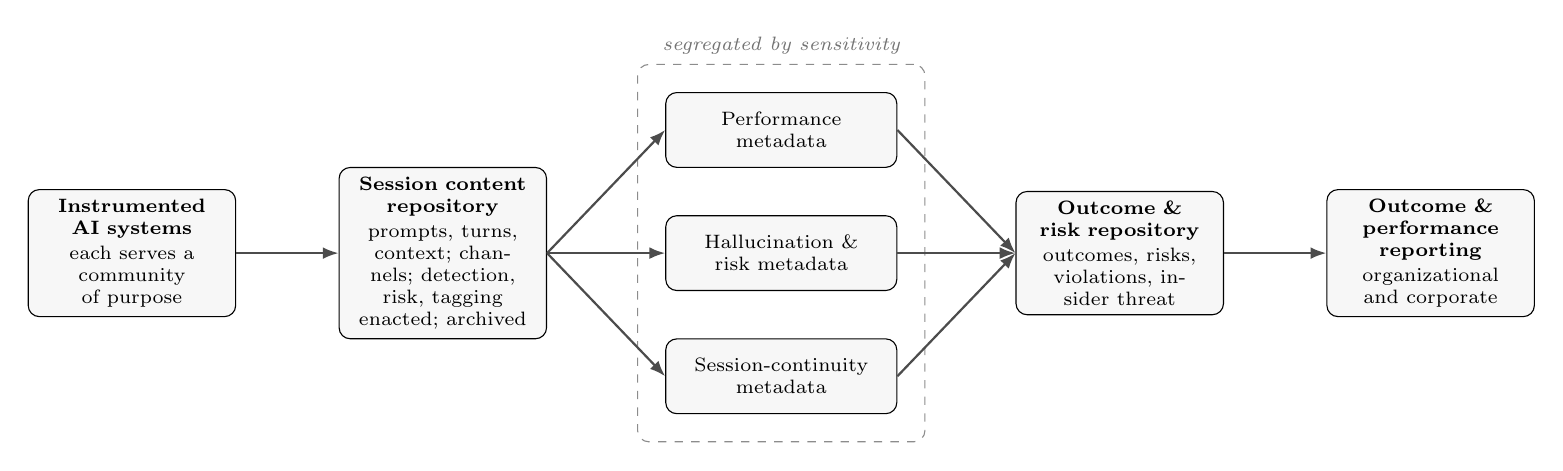
\begin{tikzpicture}[
  box/.style={draw, rounded corners, align=center, minimum height=1.25cm,
              text width=2.4cm, font=\scriptsize, fill=black!3},
  meta/.style={draw, rounded corners, align=center, minimum height=0.95cm,
               text width=2.7cm, font=\scriptsize, fill=black!3},
  arr/.style={-{Latex[length=2mm]}, thick, black!70},
  lbl/.style={font=\scriptsize\itshape, text=black!55},
  node distance=6mm and 13mm
]
\node[box] (sys) {\textbf{Instrumented AI systems}\\[1pt]each serves a community of purpose};
\node[box, right=of sys] (scr) {\textbf{Session content repository}\\[1pt]prompts, turns, context; channels; detection, risk, tagging enacted; archived};
\node[meta, right=15mm of scr] (m2) {Hallucination \& risk metadata};
\node[meta, above=of m2] (m1) {Performance metadata};
\node[meta, below=of m2] (m3) {Session-continuity metadata};
\node[box, right=15mm of m2] (out) {\textbf{Outcome \& risk repository}\\[1pt]outcomes, risks, violations, insider threat};
\node[box, right=of out] (rep) {\textbf{Outcome \& performance reporting}\\[1pt]organizational and corporate};
\node[draw, dashed, rounded corners, black!45, fit=(m1)(m2)(m3), inner sep=3.5mm,
      label={[lbl]above:segregated by sensitivity}] (mg) {};
\draw[arr] (sys) -- (scr);
\draw[arr] (scr.east) -- (m1.west);
\draw[arr] (scr.east) -- (m2.west);
\draw[arr] (scr.east) -- (m3.west);
\draw[arr] (m1.east) -- (out.west);
\draw[arr] (m2.east) -- (out.west);
\draw[arr] (m3.east) -- (out.west);
\draw[arr] (out) -- (rep);
\end{tikzpicture}
}.
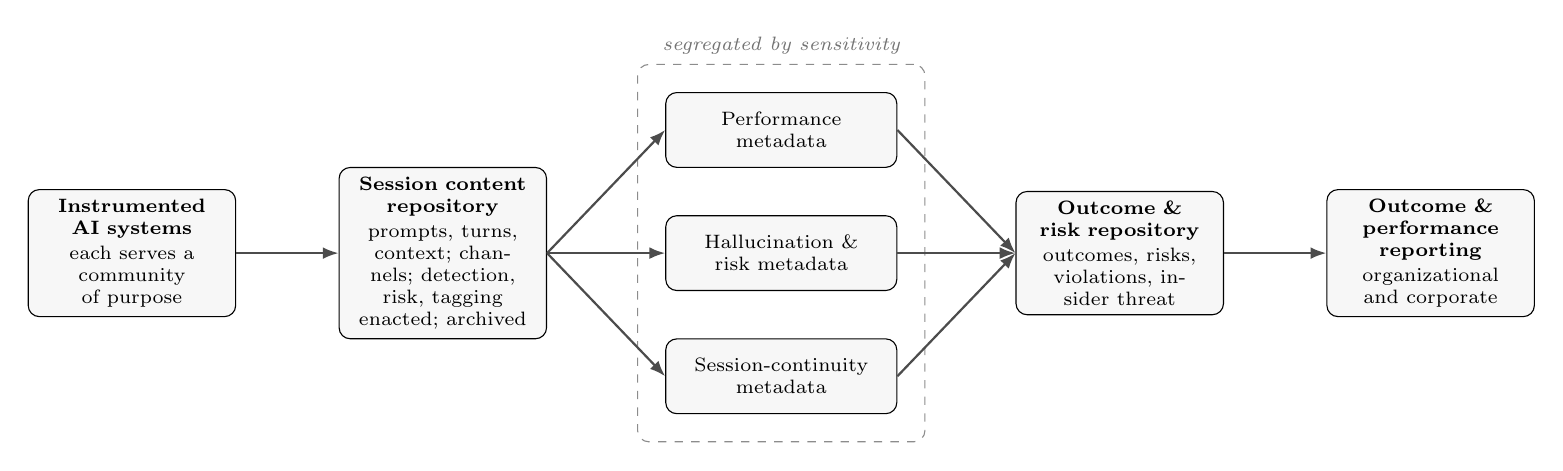
\begin{tikzpicture}[
  box/.style={draw, rounded corners, align=center, minimum height=1.25cm,
              text width=2.4cm, font=\scriptsize, fill=black!3},
  meta/.style={draw, rounded corners, align=center, minimum height=0.95cm,
               text width=2.7cm, font=\scriptsize, fill=black!3},
  arr/.style={-{Latex[length=2mm]}, thick, black!70},
  lbl/.style={font=\scriptsize\itshape, text=black!55},
  node distance=6mm and 13mm
]
\node[box] (sys) {\textbf{Instrumented AI systems}\\[1pt]each serves a community of purpose};
\node[box, right=of sys] (scr) {\textbf{Session content repository}\\[1pt]prompts, turns, context; channels; detection, risk, tagging enacted; archived};
\node[meta, right=15mm of scr] (m2) {Hallucination \& risk metadata};
\node[meta, above=of m2] (m1) {Performance metadata};
\node[meta, below=of m2] (m3) {Session-continuity metadata};
\node[box, right=15mm of m2] (out) {\textbf{Outcome \& risk repository}\\[1pt]outcomes, risks, violations, insider threat};
\node[box, right=of out] (rep) {\textbf{Outcome \& performance reporting}\\[1pt]organizational and corporate};
\node[draw, dashed, rounded corners, black!45, fit=(m1)(m2)(m3), inner sep=3.5mm,
      label={[lbl]above:segregated by sensitivity}] (mg) {};
\draw[arr] (sys) -- (scr);
\draw[arr] (scr.east) -- (m1.west);
\draw[arr] (scr.east) -- (m2.west);
\draw[arr] (scr.east) -- (m3.west);
\draw[arr] (m1.east) -- (out.west);
\draw[arr] (m2.east) -- (out.west);
\draw[arr] (m3.east) -- (out.west);
\draw[arr] (out) -- (rep);
\end{tikzpicture}
}.
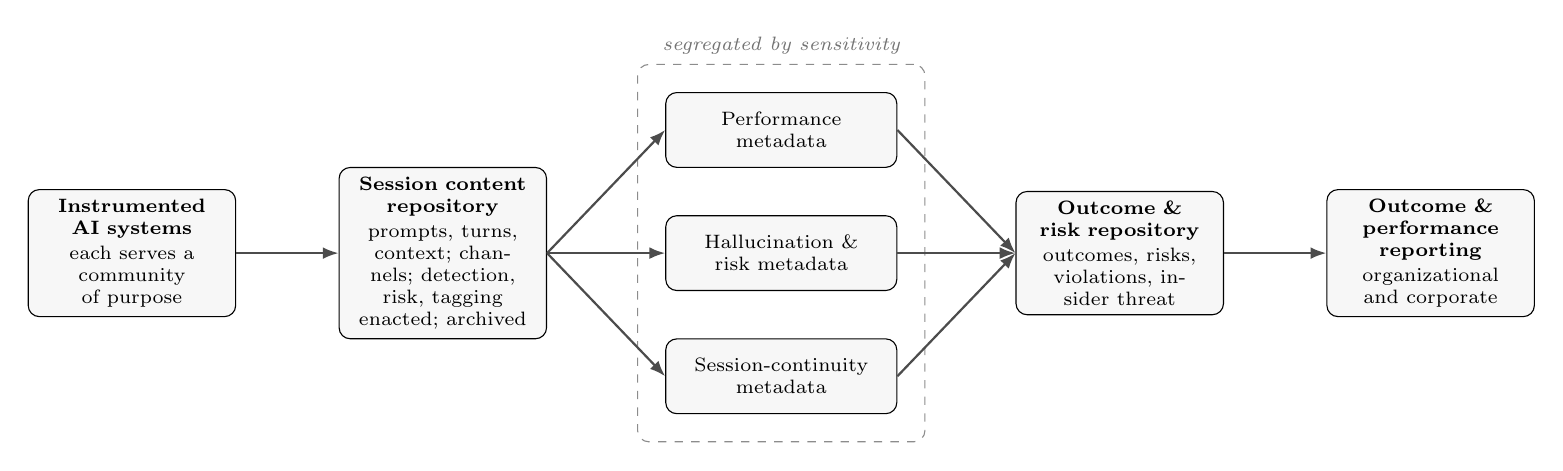
\begin{tikzpicture}[
  box/.style={draw, rounded corners, align=center, minimum height=1.25cm,
              text width=2.4cm, font=\scriptsize, fill=black!3},
  meta/.style={draw, rounded corners, align=center, minimum height=0.95cm,
               text width=2.7cm, font=\scriptsize, fill=black!3},
  arr/.style={-{Latex[length=2mm]}, thick, black!70},
  lbl/.style={font=\scriptsize\itshape, text=black!55},
  node distance=6mm and 13mm
]
\node[box] (sys) {\textbf{Instrumented AI systems}\\[1pt]each serves a community of purpose};
\node[box, right=of sys] (scr) {\textbf{Session content repository}\\[1pt]prompts, turns, context; channels; detection, risk, tagging enacted; archived};
\node[meta, right=15mm of scr] (m2) {Hallucination \& risk metadata};
\node[meta, above=of m2] (m1) {Performance metadata};
\node[meta, below=of m2] (m3) {Session-continuity metadata};
\node[box, right=15mm of m2] (out) {\textbf{Outcome \& risk repository}\\[1pt]outcomes, risks, violations, insider threat};
\node[box, right=of out] (rep) {\textbf{Outcome \& performance reporting}\\[1pt]organizational and corporate};
\node[draw, dashed, rounded corners, black!45, fit=(m1)(m2)(m3), inner sep=3.5mm,
      label={[lbl]above:segregated by sensitivity}] (mg) {};
\draw[arr] (sys) -- (scr);
\draw[arr] (scr.east) -- (m1.west);
\draw[arr] (scr.east) -- (m2.west);
\draw[arr] (scr.east) -- (m3.west);
\draw[arr] (m1.east) -- (out.west);
\draw[arr] (m2.east) -- (out.west);
\draw[arr] (m3.east) -- (out.west);
\draw[arr] (out) -- (rep);
\end{tikzpicture}
}
\caption{The architecture as a simple flow. Instrumented AI systems emit session
content to the session content repository, where channels arise and detection,
risk, and tagging are enacted. Derived metadata is separated by sensitivity into
performance, hallucination-and-risk, and session-continuity repositories.
Outcomes and risks are drawn into the outcome and risk repository and presented by
outcome and performance reporting. Every record is attributable by organization,
product line, and purpose.}
\label{fig:arch}
\end{figure}

\subsection{Instrumented systems}

The organization runs AI systems, each serving a community of purpose. Every such
system is instrumented for utilization: customer journey, throughput, user and
session counts, session context-window use, and compaction, among others. This
instrumentation is the source of the performance picture. Because each system
serves a purpose, its data is attributable to the organization and product line it
serves and aggregable by purpose and product. The set of instrumented systems,
identified by purpose and product, is the organization's live inventory of
deployed AI.

\subsection{Session content repository}

The session content repository holds the session data itself: the system and
session prompts, the human and model turns, and the session context. Channels
arise here, organized by mission and purpose, and a user's session context
supports the several swimlanes that user occupies within a system. Hallucination
detection, risk detection, and taxonomy tagging of mission data are enacted on
this content, because they operate on what was said, and the content is stored and
archived as the system of record.

\subsection{Segregated metadata repositories}

Metadata is derived from session content into repositories separated by
sensitivity, and the separation is deliberate. Performance metadata, the
utilization and throughput picture, is one repository. Hallucination and risk
metadata is a separate repository, because it is corporate-sensitive and must not
be comingled with performance reporting. Session-continuity metadata, the user
session data that a later continuity capability would reinject, is segregated
again, along boundaries of purpose, product, and organizational sensitivity,
because it is mission-centric. Separating by sensitivity, rather than gathering
everything into one store, is what lets the sensitive records be governed on their
own terms (Section~\ref{sec:governance}).

\subsection{Outcome and reporting}

The outcome and risk repository draws the positive and negative outcomes
associated with AI use, together with the hallucination and risk reporting
retrieved from the session-data metadata. It is the store of consequence of
Section~\ref{sec:measurement}. Above it, outcome and performance reporting
retrieves statistics from the metadata repositories and presents organizational
and corporate performance. This is the dashboard and the overall performance
reporting system, reporting against the layered objectives of
Section~\ref{sec:measurement} and attributing performance to organizations and
product lines.

Each part is a drill-down. The lower parts preserve and organize the record, the
upper parts interrogate and report it, and Section~\ref{sec:epistemology} argued
that the record has to come first and be kept whole.

% ---------------------------------------------------------------------------
\section{Data Model}
\label{sec:datamodel}

The data model follows from the epistemology of Section~\ref{sec:epistemology}.
If an instance's meaning is knowable only through its cause and its trajectory,
then the unit of capture cannot be a flat log line. It has to be a first-class,
immutable event that carries enough context to be explained after the fact and
linked to what came before and after it.

\subsection{The captured event}

Each interaction between a user and a generative model is stored as one
immutable event. An event records the exchanged text and the conditions that
produced it, because a response is interpretable only against the instruction
frame and the sampling regime that generated it. A hallucination produced at a
high sampling temperature under a permissive system prompt is a different event,
with a different cause, from the same surface text produced at temperature zero
under a constraining one. Recording the output without its generating conditions
discards the causal information the repository exists to preserve.

Table~\ref{tab:fields} lists the captured fields. The user identifier is a
stable pseudonymous handle, not personal data. It supports per-user measures of
utilization and acumen (Section~\ref{sec:measurement}) and workplace monitoring
of system use, while the repository avoids storing personal identifiers.
Section~\ref{sec:governance} describes the governance that keeps identity
trackable to a role and a workflow without retaining personally identifiable
information. Every field is tagged and searchable, so events can be retrieved by
user, workflow, model, system prompt, sampling regime, or content.

\begin{table}[t]
\centering
\small
\begin{tabular}{lp{0.62\linewidth}}
\toprule
Group & Captured fields \\
\midrule
Identity and routing & pseudonymous user id; workflow (lane) id; session id; tenant or organization; timestamp \\
Model configuration & model id and version; system prompt; decoding parameters (temperature, top-$p$, max tokens); available tool and function definitions \\
Interaction content & user prompt (turn); model response; tool calls and results; human interactions (edit, acceptance, rejection, follow-up) \\
Derived and links & tags; token counts; latency; cost; links to antecedent and consequent events \\
\bottomrule
\end{tabular}
\caption{Fields captured per event. Recording the generating conditions, not
only the exchanged text, is what makes an event explicable after the fact.}
\label{tab:fields}
\end{table}

\subsection{Immutability, provenance, and links}

Events are immutable and versioned. A later re-classification of an event adds a
labeled interpretation without altering the original record, so a lens built
after capture can be applied without destroying the data it reads. Each event
carries directed links to its antecedents and consequents, so a chain of
exchanges, and a cascade of failures, can be traversed rather than inferred.
Section~\ref{sec:risk} uses these links to trace recurrence and causality.

The repository keeps each record in two forms. A raw, append-only form preserves
each interaction exactly as captured and is never rewritten. A structured form
makes the fields of Table~\ref{tab:fields} queryable at scale and carries the
links between records, so a chain of exchanges, and a cascade of failures, can be
followed by query. Linkage is a property of the records, not a separate store.
Figure~\ref{fig:datamodel} shows the two forms and how records link across
channels.

\begin{figure}[t]
\centering
\resizebox{\textwidth}{!}{% Figure F2 --- the data model: two forms of each record, plus typed linked channels.
% Included from main.tex via \resizebox{\textwidth}{!}{% Figure F2 --- the data model: two forms of each record, plus typed linked channels.
% Included from main.tex via \resizebox{\textwidth}{!}{% Figure F2 --- the data model: two forms of each record, plus typed linked channels.
% Included from main.tex via \resizebox{\textwidth}{!}{\input{fig2_data_model}}.
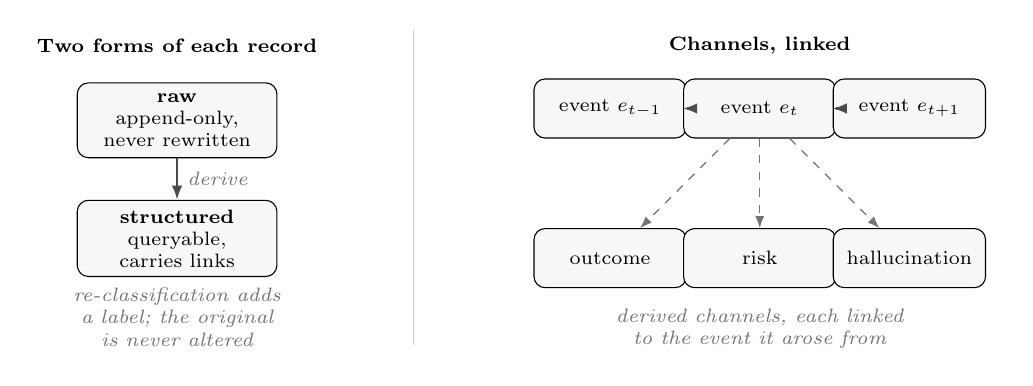
\begin{tikzpicture}[
  rec/.style={draw, rounded corners, align=center, minimum height=0.75cm,
              text width=1.7cm, font=\scriptsize, fill=black!3},
  form/.style={draw, rounded corners, align=center, minimum height=0.95cm,
               text width=2.3cm, font=\scriptsize, fill=black!3},
  arr/.style={-{Latex[length=1.8mm]}, thick, black!70},
  xlink/.style={-{Latex[length=1.5mm]}, dashed, black!55},
  ttl/.style={font=\scriptsize\bfseries},
  lbl/.style={font=\scriptsize\itshape, text=black!55}
]
% ----- Panel A: two forms -----
\node[ttl] at (1.4,2.3) {Two forms of each record};
\node[form] (raw) at (1.4,1.35) {\textbf{raw}\\append-only,\\never rewritten};
\node[form] (str) at (1.4,-0.15) {\textbf{structured}\\queryable,\\carries links};
\draw[arr] (raw) -- node[right,lbl]{derive} (str);
\node[lbl, align=center, text width=3cm] at (1.4,-1.15)
     {re-classification adds a label; the original is never altered};
% ----- divider -----
\draw[black!20] (4.4,-1.5) -- (4.4,2.5);
% ----- Panel B: channels + links -----
\node[ttl] at (8.8,2.3) {Channels, linked};
\node[rec] (e1) at (6.9,1.5) {event $e_{t-1}$};
\node[rec] (e2) at (8.8,1.5) {event $e_t$};
\node[rec] (e3) at (10.7,1.5) {event $e_{t+1}$};
\draw[arr] (e1) -- (e2);
\draw[arr] (e2) -- (e3);
\node[rec] (o) at (6.9,-0.4) {outcome};
\node[rec] (r) at (8.8,-0.4) {risk};
\node[rec] (h) at (10.7,-0.4) {hallucination};
\draw[xlink] (e2) -- (o);
\draw[xlink] (e2) -- (r);
\draw[xlink] (e2) -- (h);
\node[lbl, align=center, text width=6cm] at (8.8,-1.3)
     {derived channels, each linked to the event it arose from};
\end{tikzpicture}
}.
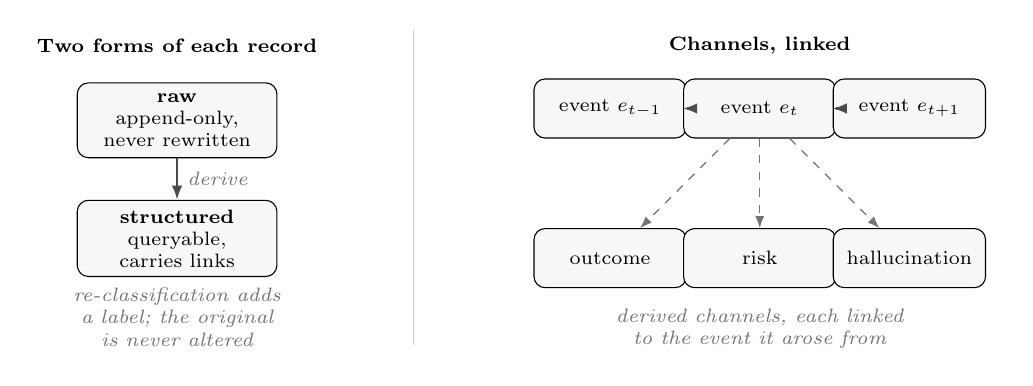
\begin{tikzpicture}[
  rec/.style={draw, rounded corners, align=center, minimum height=0.75cm,
              text width=1.7cm, font=\scriptsize, fill=black!3},
  form/.style={draw, rounded corners, align=center, minimum height=0.95cm,
               text width=2.3cm, font=\scriptsize, fill=black!3},
  arr/.style={-{Latex[length=1.8mm]}, thick, black!70},
  xlink/.style={-{Latex[length=1.5mm]}, dashed, black!55},
  ttl/.style={font=\scriptsize\bfseries},
  lbl/.style={font=\scriptsize\itshape, text=black!55}
]
% ----- Panel A: two forms -----
\node[ttl] at (1.4,2.3) {Two forms of each record};
\node[form] (raw) at (1.4,1.35) {\textbf{raw}\\append-only,\\never rewritten};
\node[form] (str) at (1.4,-0.15) {\textbf{structured}\\queryable,\\carries links};
\draw[arr] (raw) -- node[right,lbl]{derive} (str);
\node[lbl, align=center, text width=3cm] at (1.4,-1.15)
     {re-classification adds a label; the original is never altered};
% ----- divider -----
\draw[black!20] (4.4,-1.5) -- (4.4,2.5);
% ----- Panel B: channels + links -----
\node[ttl] at (8.8,2.3) {Channels, linked};
\node[rec] (e1) at (6.9,1.5) {event $e_{t-1}$};
\node[rec] (e2) at (8.8,1.5) {event $e_t$};
\node[rec] (e3) at (10.7,1.5) {event $e_{t+1}$};
\draw[arr] (e1) -- (e2);
\draw[arr] (e2) -- (e3);
\node[rec] (o) at (6.9,-0.4) {outcome};
\node[rec] (r) at (8.8,-0.4) {risk};
\node[rec] (h) at (10.7,-0.4) {hallucination};
\draw[xlink] (e2) -- (o);
\draw[xlink] (e2) -- (r);
\draw[xlink] (e2) -- (h);
\node[lbl, align=center, text width=6cm] at (8.8,-1.3)
     {derived channels, each linked to the event it arose from};
\end{tikzpicture}
}.
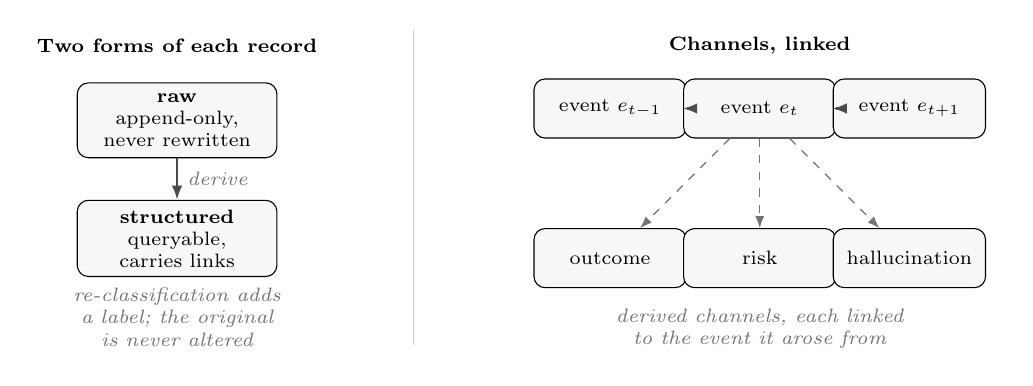
\begin{tikzpicture}[
  rec/.style={draw, rounded corners, align=center, minimum height=0.75cm,
              text width=1.7cm, font=\scriptsize, fill=black!3},
  form/.style={draw, rounded corners, align=center, minimum height=0.95cm,
               text width=2.3cm, font=\scriptsize, fill=black!3},
  arr/.style={-{Latex[length=1.8mm]}, thick, black!70},
  xlink/.style={-{Latex[length=1.5mm]}, dashed, black!55},
  ttl/.style={font=\scriptsize\bfseries},
  lbl/.style={font=\scriptsize\itshape, text=black!55}
]
% ----- Panel A: two forms -----
\node[ttl] at (1.4,2.3) {Two forms of each record};
\node[form] (raw) at (1.4,1.35) {\textbf{raw}\\append-only,\\never rewritten};
\node[form] (str) at (1.4,-0.15) {\textbf{structured}\\queryable,\\carries links};
\draw[arr] (raw) -- node[right,lbl]{derive} (str);
\node[lbl, align=center, text width=3cm] at (1.4,-1.15)
     {re-classification adds a label; the original is never altered};
% ----- divider -----
\draw[black!20] (4.4,-1.5) -- (4.4,2.5);
% ----- Panel B: channels + links -----
\node[ttl] at (8.8,2.3) {Channels, linked};
\node[rec] (e1) at (6.9,1.5) {event $e_{t-1}$};
\node[rec] (e2) at (8.8,1.5) {event $e_t$};
\node[rec] (e3) at (10.7,1.5) {event $e_{t+1}$};
\draw[arr] (e1) -- (e2);
\draw[arr] (e2) -- (e3);
\node[rec] (o) at (6.9,-0.4) {outcome};
\node[rec] (r) at (8.8,-0.4) {risk};
\node[rec] (h) at (10.7,-0.4) {hallucination};
\draw[xlink] (e2) -- (o);
\draw[xlink] (e2) -- (r);
\draw[xlink] (e2) -- (h);
\node[lbl, align=center, text width=6cm] at (8.8,-1.3)
     {derived channels, each linked to the event it arose from};
\end{tikzpicture}
}
\caption{The data model. Each record is kept in two forms: a raw, append-only form
that is never rewritten, and a structured, queryable form derived from it, so a
later re-classification adds a label without altering the original. Records are
organized into typed channels (event, outcome, risk, hallucination) and linked,
both along the event channel as antecedents and consequents and across channels, so
a derived record can be read together with the event it arose from. The fields
captured per event are listed in Table~\ref{tab:fields}.}
\label{fig:datamodel}
\end{figure}

\subsection{Channels}

The session content repository is not a single stream. It is a set of channels,
each a typed, linked stream of one kind of record, organized by mission and
purpose. Session content, detections, and outcomes are distinct channels that link
to one another, so a risk can be read together with the event that raised it and
the outcome it threatens. Which repository a channel is stored in is a matter of
sensitivity, not model. Session content is archived in the session content
repository, while derived metadata is segregated into the metadata repositories of
Section~\ref{sec:architecture} by purpose, product, and sensitivity. What the
model fixes is that every channel is typed and linked, so segregating the stores
never severs the links between records.

% ---------------------------------------------------------------------------
\section{Measurement Framework}
\label{sec:measurement}

Measures of performance, measures of effectiveness, and key performance
indicators are not properties of the AI architecture. They are the strategic and
operational objectives of the organization, defined by the organization and by
the corporation above it, in layers. A corporation sets strategic objectives, a
division sets operational objectives that serve them, and a team or workflow sets
local objectives in turn. Each layer names its own measures. The architecture
does not define these measures and should not. Its role is to collect, detect,
catalog, and store the outcomes those measures are computed from, so that each
layer can report against its own objectives. Figure~\ref{fig:measurement}
summarizes the framework.

\begin{figure}[t]
\centering
\resizebox{\textwidth}{!}{% Figure F3 --- the measurement framework: layered exogenous objectives, measure
% families per layer, rolled up over the record. \resizebox to \textwidth in main.tex.
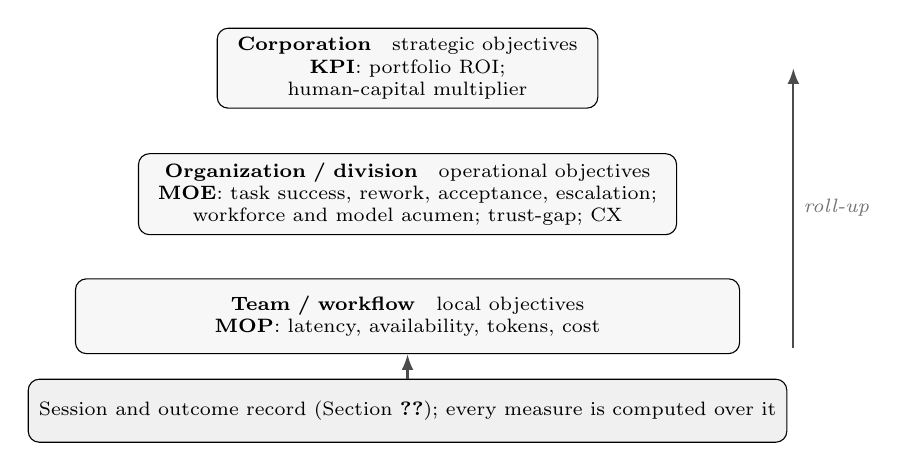
\begin{tikzpicture}[
  band/.style={draw, rounded corners, align=center, minimum height=0.95cm,
               font=\scriptsize, fill=black!3},
  base/.style={draw, rounded corners, align=center, minimum height=0.8cm,
               text width=9.4cm, font=\scriptsize, fill=black!6},
  arr/.style={-{Latex[length=2mm]}, thick, black!70},
  lbl/.style={font=\scriptsize\itshape, text=black!55}
]
\node[band, text width=8.2cm] (wf) at (5,0.2)
     {\textbf{Team / workflow} \; local objectives\\
      \textbf{MOP}: latency, availability, tokens, cost};
\node[band, text width=6.6cm] (org) at (5,1.75)
     {\textbf{Organization / division} \; operational objectives\\
      \textbf{MOE}: task success, rework, acceptance, escalation;\\
      workforce and model acumen; trust-gap; CX};
\node[band, text width=4.6cm] (corp) at (5,3.35)
     {\textbf{Corporation} \; strategic objectives\\
      \textbf{KPI}: portfolio ROI; human-capital multiplier};
\node[base] (rec) at (5,-1.0)
     {Session and outcome record (Section~\ref{sec:datamodel}); every measure is computed over it};
\draw[arr] (rec) -- (wf);
\draw[arr] (9.9,-0.2) -- node[right,lbl]{roll-up} (9.9,3.35);
\end{tikzpicture}
}
\caption{The measurement framework. Objectives are exogenous and layered: each of
the workflow, organizational, and corporate layers defines its own measures. The
architecture does not set the measures; it computes them over the session and
outcome record and rolls outcomes up the hierarchy. Measures of performance sit
close to the interaction, measures of effectiveness against the objective a
workflow serves, and key performance indicators at the business-facing top,
alongside the workforce and model acumen measures, the trust-calibration gap, and
customer experience.}
\label{fig:measurement}
\end{figure}

\subsection{Objectives are defined by the organization, in layers}

The organization owns the objective hierarchy, and the architecture holds a model
of it: a catalog of the objectives each layer has declared. A captured
interaction is associated with the objectives it bears on, and outcomes roll up
from the workflow where they occur to the strategic objective they serve. Because
the objectives are exogenous, the architecture adapts to whatever an organization
declares rather than imposing a fixed set of metrics. This is the principle of
Section~\ref{sec:epistemology} applied to measurement: the record has to support
measurement against objectives that were not anticipated when it was captured,
because an organization revises its objectives over time.

\subsection{The outcome repository}

An outcome is a realized value of a measure, attributable to AI use, at a point
in time. The architecture treats outcomes as first-class records, stored in an
outcome repository alongside the event record of Section~\ref{sec:datamodel}.
Outcomes are collected where they are declared, detected where they are implicit,
since a resolved case, an accepted draft, or a completed transaction is an
outcome the record can recognize without being told, cataloged against the
objective hierarchy, and stored so that reporting draws on a persistent, queryable
history rather than a snapshot. Because each outcome links to the interactions
that produced it, an outcome can be traced to the AI use it is credited to or
charged against.

The repository stores outcomes of both signs together with the conditions around
them. It holds positive outcomes and negative outcomes, and three classes a
measurement-only store would omit: risks, which are anticipated negative outcomes
not yet realized; violations, which are breaches of the obligations of
Section~\ref{sec:obligations}; and insider-threat indicators, which are signs
that AI is being used to act against the organization. Each is a consequence,
realized or potential, that leadership has to see and report, so each takes the
outcome record form and links back to the interactions it arose from.

Two dimensions organize the store. The first is organizational structure: an
outcome is filed against the unit it belongs to, so that the overall organization
and its internal units stay distinguishable and a unit's outcomes can be read
apart from the whole. The second is the objective it bears on, from the layered
hierarchy above, so that an outcome rolls up from the workflow where it occurred
to the strategic objective it serves. Together the two dimensions let a report be
drawn for the whole organization or for any unit, against that level's own
objectives.

The repository also records the context an outcome arose in. Outcomes from live
operation and outcomes from exercises, drills, and simulations are kept apart, so
that an organization can rehearse against the record and assess its readiness
without contaminating the measures of live performance. Insider-threat and
violation records carry the same separation, since a rehearsed exercise and a
real breach must never be counted as the same event. The governance of who may
read these records, and the privacy limits on monitoring for them, is the subject
of Section~\ref{sec:governance}.

\subsection{Performance, effectiveness, and indicators}

Within this frame the three families sit at different layers. Measures of
performance describe whether the system did the thing: latency, availability,
token use, and cost, computed close to the interaction. Measures of effectiveness
describe whether the objective was achieved: task success, rework, acceptance,
escalation, and time to deliver, computed against the objective a workflow serves.
Key performance indicators are the business-facing roll-ups each layer reports. To
these the architecture adds measures the record makes possible and a fixed
dashboard would miss: workforce acumen, computed from how skillfully users direct
and check the AI; model acumen and drift, computed from the model's reliability
over time; the trust-calibration gap of Section~\ref{sec:trust}; customer
experience for customer-facing work, in satisfaction, resolution, and escalation;
and token cost as the denominator of return. Measurement is neutral to the sign
of what it finds. The same record yields the positive and negative outcomes of
Section~\ref{sec:risk}.

\subsection{Portfolio reporting}

The AI architecture is a funded investment, and like any portfolio investment it
has to justify its cost. The measurement layer supports reporting at the level a
portfolio owner needs: what the organization spends on AI, set against the
outcomes attributable to it, reported against the objectives each layer defined.
Cost is known from the record of Section~\ref{sec:datamodel}. Outcome value is
known from the outcome repository. Return is the relation between them, reported
at each layer of the objective hierarchy. Without the record, this report is an
anecdote. With it, it is an account.

Because the record makes cost and outcome both measurable, the return on the AI
investment is calculable rather than asserted. The investment is measurable, the
deployment is instrumented, and the achievement of the workforce and the evolution
of AI's benefit over time are trackable against the objectives each layer set. The
question an executive most wants answered, how far AI multiplies human capital,
becomes a computed quantity: the output a workforce produces with AI, set against
what it produced without, tracked as it changes. Without the record none of these
is calculable, and the investment is defended by anecdote.

\subsection{Competency and mission, in both directions}

The measurement establishes how the AI architecture affects the organization's
competency and its mission deliverables, and the effect runs in both directions.
AI can raise organizational competency by completing work faster or better, and it
can lower it by displacing skills a workforce would otherwise maintain. A
workforce that defers to the model on a class of task can lose the ability to
perform or check that task, which is a degradation of competency even when
short-term output looks improved. The measurement layer has to show both, because
a portfolio owner deciding whether the investment pays needs the losses as well as
the gains. This connects to the trust of Section~\ref{sec:trust}: over-reliance is
the mechanism by which competency degrades, and it shows up in the record as
reliance that outruns verification.

% ---------------------------------------------------------------------------
\section{Outcomes: Benefit, Harm, and Liability}
\label{sec:risk}

An AI deployment produces outcomes of both signs, and the record captures them
with the same machinery. On the positive side are mission benefit and
performance improvement: work completed faster, at lower cost, or at higher
quality than before. On the negative side are error, rework, harm, and
liability. Measurement (Section~\ref{sec:measurement}) is neutral to the sign of
an outcome. What makes an outcome legible is that the interaction which produced
it, and the downstream use of its output, are on the record.

\subsection{Positive outcomes}

Performance improvement and mission benefit are measured as changes in the
measures of effectiveness of Section~\ref{sec:measurement}, attributed to AI use
through the record: which workflows use AI, how their task success, cost, and
time change, and whether the change holds. Without the record, benefit is
asserted anecdotally. With it, benefit is measured and attributed to the work
that produced it.

\subsection{Harm and the adverse-event lifecycle}

Negative outcomes follow a lifecycle borrowed from adverse-event surveillance. A
single failure is an instance. Its importance is not evident at the instant it
occurs, because impact is a function of trajectory. Repeated instances form an
incidence that can be tracked. Some instances trace to a cause, and some cascade
into further failures downstream. A mitigation applied after detection has an
efficacy that is itself measurable, as a change in incidence across a dated
boundary, and a mitigation moved upstream becomes prevention. Each step is a
query over the linked record of Section~\ref{sec:datamodel}, not an inference
from a point-in-time log. Figure~\ref{fig:lifecycle} shows the lifecycle.

\begin{figure}[t]
\centering
\resizebox{\textwidth}{!}{% Figure F4 --- the hallucination adverse-event lifecycle (Section 8).
% \resizebox to \textwidth in main.tex.
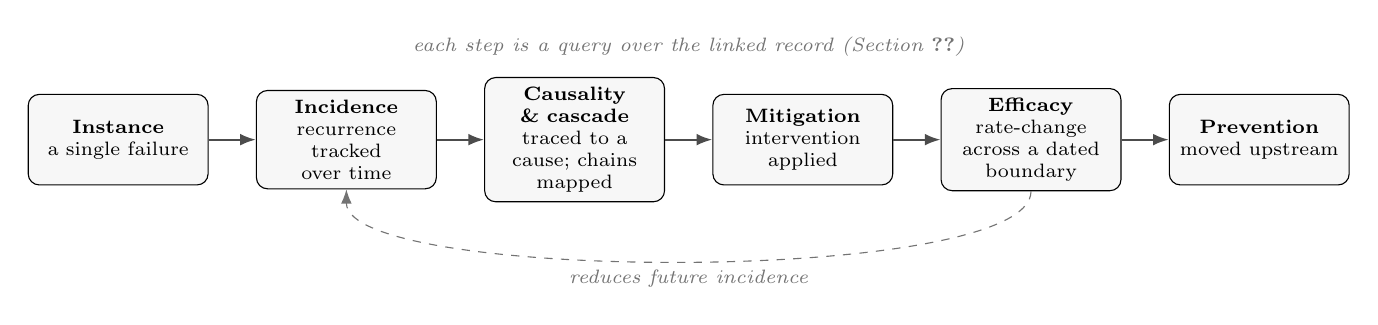
\begin{tikzpicture}[
  st/.style={draw, rounded corners, align=center, minimum height=1.15cm,
             text width=2.05cm, font=\scriptsize, fill=black!3},
  arr/.style={-{Latex[length=2mm]}, thick, black!70},
  fb/.style={-{Latex[length=1.8mm]}, dashed, black!55},
  lbl/.style={font=\scriptsize\itshape, text=black!55},
  node distance=6mm
]
\node[st] (s1) {\textbf{Instance}\\a single failure};
\node[st, right=of s1] (s2) {\textbf{Incidence}\\recurrence tracked over time};
\node[st, right=of s2] (s3) {\textbf{Causality \& cascade}\\traced to a cause; chains mapped};
\node[st, right=of s3] (s4) {\textbf{Mitigation}\\intervention applied};
\node[st, right=of s4] (s5) {\textbf{Efficacy}\\rate-change across a dated boundary};
\node[st, right=of s5] (s6) {\textbf{Prevention}\\moved upstream};
\draw[arr] (s1) -- (s2);
\draw[arr] (s2) -- (s3);
\draw[arr] (s3) -- (s4);
\draw[arr] (s4) -- (s5);
\draw[arr] (s5) -- (s6);
\draw[fb] (s5.south) to[out=-90,in=-90,looseness=0.35]
     node[below,lbl]{reduces future incidence} (s2.south);
\node[lbl] at ($(s1.north)!0.5!(s6.north)+(0,6mm)$)
     {each step is a query over the linked record (Section~\ref{sec:datamodel})};
\end{tikzpicture}
}
\caption{The hallucination lifecycle, adapted from adverse-event surveillance. A
single instance recurs into a tracked incidence, is traced to a cause and its
cascade, and draws a mitigation whose efficacy is measured as a change in
incidence across the dated boundary at which it was applied; an effective
mitigation moved upstream becomes prevention and reduces future incidence. Each
step is a query over the linked record, not an inference from a point-in-time log.}
\label{fig:lifecycle}
\end{figure}

\subsection{A working taxonomy of hallucination}

Harm has structure. The failures grouped under the word hallucination are not one
thing, and detecting them requires knowing which form is in play. The repository
classifies hallucination against a working taxonomy, summarized in
Table~\ref{tab:taxonomy}. The taxonomy matters to the architecture in a specific
way. Each category is detectable only from particular captured fields, so the
taxonomy is the reason the data model of Section~\ref{sec:datamodel} records the
generating conditions, the provenance, and the session trajectory, and not the
output alone. The categories synthesize forms recognized in the
hallucination-detection literature \cite{ji2023hallucination} with operational
forms specific to deployed and agentic systems.

\begin{table}[t]
\centering
\small
\begin{tabular}{p{0.20\linewidth}p{0.40\linewidth}p{0.28\linewidth}}
\toprule
Category & How it appears in use & Repository signal \\
\midrule
Fabrication & Asserts a fact, source, feature, or justification that is not true or not grounded & Output checked against provenance; assertions with no grounded source \\
Overconfidence and misrepresentation & Asserts without verification, or reports a task as done or correct when it is partial or untested & Confidence and completion claims vs verification steps and downstream outcome \\
Staleness & Treats outdated information as current, or omits a freshness check & Cited sources and state vs their capture time and current values \\
Context loss & As a session lengthens or crosses a boundary, drops, reshapes, or forgets earlier content & Session trajectory and context-window use; later output vs earlier record \\
Attribution error & Misassigns a source, an authority, or a capability & Claimed attributions vs provenance links \\
Scope and instruction divergence & Does more than, or other than, what was asked & Output scope vs the recorded prompt and workflow boundary \\
Agentic and tool-use failure & Acts without verifying preconditions, misuses or ignores a tool, references a resource that does not exist, or takes an unsafe action & Tool calls, preconditions, and referenced resources vs the recorded environment \\
\bottomrule
\end{tabular}
\caption{A working taxonomy of hallucination the repository is designed to
characterize and detect. Categories are not mutually exclusive; a single event
can carry more than one. Applicable categories depend on how the organization
uses AI.}
\label{tab:taxonomy}
\end{table}

Fabrication is treated at greater length next, because it is the form most
damaging to an organization's fact base.

\subsection{Fabrication masquerading as fact}

The sharpest harm is specific to generative systems. A hallucination is not only
a wrong answer. It is fiction presented in the form of established fact, fluent
and confident, and once it enters an organization's records it can corrupt the
fact base that later work depends on. The architectural defense is provenance.
Because every event carries the conditions and source of its content
(Section~\ref{sec:datamodel}), a generated assertion stays distinguishable from a
curated fact. The repository does not prevent fabrication at the moment of
generation. It prevents fabrication from silently becoming fact, by preserving
the boundary between what a model asserted and what was established as true.

\subsection{Liability}

Negative outcomes carry liability, and liability attaches to specific acts.
Establishing what the model was asked, under what configuration, what it
produced, who relied on it, and what followed requires exactly the record this
paper describes. The obligations that an outcome may violate, and against which
liability is assessed, are the subject of Section~\ref{sec:obligations}.

% ---------------------------------------------------------------------------
\section{Obligations: What AI Must Be Evaluated Against}
\label{sec:obligations}

An AI output or action is not evaluated against correctness alone. It is
evaluated against the obligations that bind the person or organization that used
it. An answer can be factually right and still violate a policy, a law, a
professional standard, or a required procedure. To manage AI, an organization has
to evaluate its use against each class of obligation that applies, and that
evaluation is possible only over a record that holds the output together with its
conditions and its downstream use.

Table~\ref{tab:obligations} gives a sample set of obligation classes. The set is
not exhaustive, and which classes apply depends on the domain, but the classes
are general enough to frame the evaluation for most deployments.

\begin{table}[t]
\centering
\small
\begin{tabular}{p{0.17\linewidth}p{0.42\linewidth}p{0.29\linewidth}}
\toprule
Class & What it obliges & Example failure \\
\midrule
Organizational & Internal policy, brand and communication standards, role and workflow scope & Acting outside an authorized workflow \\
Legal and regulatory & Statute, regulation, contract and licensing terms, intellectual property, data protection & Reproducing licensed text; mishandling regulated data \\
Ethical & Fairness, non-deception, non-maleficence, transparency, avoidance of bias & Biased screening; undisclosed automation \\
Procedural & Required process, review gates, verification and citation, documentation & Skipping a mandated human review or source check \\
Professional and domain & The standard of care and competence of the profession or domain & Advice below a professional standard \\
Factual and epistemic & Grounding in established fact, provenance, non-fabrication & Fabrication presented as fact (Section~\ref{sec:risk}) \\
Safety and operational & Avoidance of harmful action, security, reliability & An unsafe automated action \\
\bottomrule
\end{tabular}
\caption{A sample set of obligation classes an AI use can be evaluated against.
The set is not exhaustive; applicable classes depend on the domain.}
\label{tab:obligations}
\end{table}

The repository makes each of these evaluations possible for the same reason.
Conformance and violation are both properties of a recorded interaction and its
consequences, and neither can be assessed for an interaction that was never
captured. Evaluation against obligations is a use of the record, and a violation
is one of the negative outcomes of Section~\ref{sec:risk}.

% ---------------------------------------------------------------------------
\section{Trust as an Earned Property}
\label{sec:trust}

Trust is central to AI deployment, and it is the property most likely to be
misplaced. Users tend to treat an AI as an expert. Unless they are trained
otherwise, they attribute expertise and authority to it that it has not earned,
and they extend trust its record does not justify. Fluent, confident output
invites this. The result is unwarranted trust, and it is dangerous precisely
because the system's failures, as Section~\ref{sec:risk} described, arrive in the
form of confident fact.

Trust should instead be calibrated. Reliance on the AI should track its
demonstrated reliability. Trust that exceeds reliability is over-trust, and it
turns each fabrication into an accepted fact. Trust that falls short of
reliability is under-trust, and it forfeits benefit the AI could provide. The
goal is not maximal trust or minimal trust but reliance that matches evidence.

Calibration requires two things the repository provides. Trust has to be earned,
which means measured: the reliability of the AI on a task, a workflow, or a class
of question is a statistic computed over the record, not an impression. And trust
has to be curated, which means surfaced: the provenance of an output, the model's
track record on similar work, and the confidence attached to an assertion have to
be presented to the user, so that reliance tracks evidence rather than fluency. A
user who can see that an assertion is a generated claim without a source, on a
task where the model has a poor record, is a user who can withhold trust that has
not been earned.

Managed this way, trust becomes a property the deployment measures and cultivates
rather than a disposition users bring by default. This connects the workforce
acumen of Section~\ref{sec:measurement}, since a habitually over-trusting user is
a measurable risk, to the obligations of Section~\ref{sec:obligations}, since
misplaced trust is how an obligation violation reaches a consequence unchecked.

% ---------------------------------------------------------------------------
\section{Theory of Operation}
\label{sec:operation}

The architecture is deployed as a client-side system that captures at the points
of AI use, stores to the repository, and serves reporting back to the
organization. This section describes the functional components it runs and the
topology it is deployed in, and then the continuity capability planned for a later
phase. Figure~\ref{fig:deployment} shows the deployment.

\begin{figure}[t]
\centering
\resizebox{\textwidth}{!}{% Figure F5 --- client deployment: instrumentation points feeding the repository,
% with the health-and-availability monitor. \resizebox to \textwidth in main.tex.
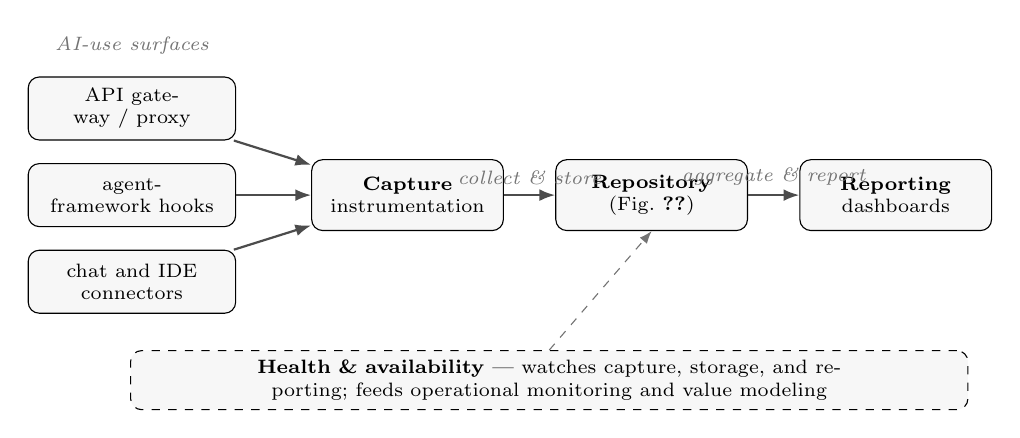
\begin{tikzpicture}[
  box/.style={draw, rounded corners, align=center, minimum height=0.9cm,
              text width=2.2cm, font=\scriptsize, fill=black!3},
  surf/.style={draw, rounded corners, align=center, minimum height=0.8cm,
               text width=2.4cm, font=\scriptsize, fill=black!3},
  arr/.style={-{Latex[length=2mm]}, thick, black!70},
  obs/.style={-{Latex[length=1.6mm]}, dashed, black!55},
  lbl/.style={font=\scriptsize\itshape, text=black!55}
]
% AI-use surfaces (left)
\node[surf] (su1) at (0,2.2) {API gateway / proxy};
\node[surf] (su2) at (0,1.1) {agent-framework hooks};
\node[surf] (su3) at (0,0.0) {chat and IDE connectors};
\node[lbl] at (0,3.0) {AI-use surfaces};
% pipeline
\node[box] (cap) at (3.5,1.1) {\textbf{Capture}\\instrumentation};
\node[box] (repo) at (6.6,1.1) {\textbf{Repository}\\(Fig.~\ref{fig:arch})};
\node[box] (rep) at (9.7,1.1) {\textbf{Reporting}\\dashboards};
\draw[arr] (su1) -- (cap);
\draw[arr] (su2) -- (cap);
\draw[arr] (su3) -- (cap);
\draw[arr] (cap) -- node[above,lbl]{collect \& store} (repo);
\draw[arr] (repo) -- node[above,lbl]{aggregate \& report} (rep);
% health & availability band
\node[draw, dashed, rounded corners, fill=black!3, align=center, text width=10.4cm,
      minimum height=0.75cm, font=\scriptsize] (hb) at (5.3,-1.25)
     {\textbf{Health \& availability} --- watches capture, storage, and reporting;
      feeds operational monitoring and value modeling};
\draw[obs] (hb.north) -- (repo.south);
\end{tikzpicture}
}
\caption{Client deployment. Instrumentation at the AI-use surfaces, an API gateway
or proxy, hooks in agent frameworks, and connectors to chat and development
interfaces, captures each interaction and collects it to the repository, which is
then aggregated and served as reporting. A health-and-availability monitor watches
capture, storage, and reporting, and feeds both operational monitoring and value
modeling, because an observability system has to be observable.}
\label{fig:deployment}
\end{figure}

\subsection{Functional components}

Three functional components run across the parts of
Section~\ref{sec:architecture}. The first collects and stores: it ingests each
interaction and outcome and persists it to the channels of
Section~\ref{sec:datamodel}. The second aggregates and reports: it rolls records
up the objective hierarchy and the organizational structure and serves the reports
of Section~\ref{sec:measurement}. The third monitors health and availability: it
watches whether capture, storage, and reporting are themselves working, because an
observability system has to be observable. Its output serves two ends. It drives
operational monitoring, so that an outage in capture is seen rather than mistaken
for an absence of activity, and it feeds value modeling, since availability is
part of the value an organization receives and downtime is value it does not.

\subsection{Deployment topology: convergence and isolation}

The channels of Section~\ref{sec:datamodel} can be converged into one repository
with logical separation, or split into isolated systems, and the choice is a
matter of assurance. Where separation is a convenience, convergence with the
context and structure dimensions of Section~\ref{sec:measurement} is enough. Where
separation has to be guaranteed, the systems are isolated rather than converged.
Live operation and exercises can run on separate systems, so that a drill cannot
spill into live measures and a live incident cannot enter a rehearsal. A sensitive
organizational product line can run on its own isolated system, so that its record
cannot contaminate, or be contaminated by, the rest. Isolation trades the
convenience of a single store for a guarantee that certain records never meet, and
an organization chooses, per population, which guarantee it needs.

\subsection{Future leg: controlled continuity and workflow isolation}
\label{sec:continuity}

A later phase of the system adds two capabilities that share one principle:
context should move between sessions only under explicit control.

The first is continuity reinjection. Because a session's record is preserved in
full, a later session can be resumed by re-injecting a curated summary of the
prior one, so that work continues across the session boundary rather than
restarting at it. The reinjected context is drawn from the record, is itself
recorded, and is scoped to the workflow it belongs to.

The second is workflow isolation. A single user runs several distinct workflows,
and these must not intermingle. The system gives each user a set of isolated
lanes, and a session is bound to one lane. Continuity reinjection draws only from
the lane's own history, and one lane's context cannot leak into another.
Isolation is not only an organizational convenience. Uncontrolled mixing of
unrelated context is itself a source of error in generative systems, because a
model conditioned on material from an unrelated task will draw on it. Binding a
session to a lane makes continuity deliberate and bounds the context a response
can be conditioned on.

Together these turn session continuity from an accident of whatever remains in a
context window into a governed operation. Continuity is restored on purpose, from
the record, within a boundary.

% ---------------------------------------------------------------------------
\section{Registered Predictions}
\label{sec:predictions}

This is a proposal, and its claims will be tested by deployment rather than by
results reported here. To make that test meaningful, we state the paper's central
predictions now, as specific and falsifiable claims, so that later observation in
deployed systems can confirm or refute them against the dated record. Each
prediction follows from the theory of operation and is checkable from the kind of
data the architecture captures.

\begin{enumerate}
\item Hallucination recurrence for a given type clusters in time around
context-window saturation and compaction events, rather than arriving at random.
\item In a corpus captured broadly, the rate at which newly detectable failure
classes appear rises with the age and size of the corpus, because detection is
retrospective and emergent (Section~\ref{sec:epistemology}).
\item The efficacy of a mitigation is measurable as a change in incidence across
the dated boundary at which it was applied, and the effect either persists or
decays measurably over the sessions that follow.
\item Without a repository, the impact of an incident is systematically
underestimated, because the cascade linking it to its consequences is not
observable at the moment the incident occurs.
\item Workforce acumen, measured from correction cadence and instruction
specificity, correlates with realized measures of effectiveness independently of
the capability of the model in use.
\item A change to the capture schema creates a permanent retrospective blind spot,
observable afterward as a discontinuity in a metric that was trackable before the
change.
\end{enumerate}

We record these as of the date of this paper, so that their confirmation, if it
comes, is a matter of record and not of hindsight.

% ---------------------------------------------------------------------------
\section{Governance, Privacy, and Compliance}
\label{sec:governance}

The record described in this paper is powerful because it is complete, and it is
sensitive for the same reason. Governance is what makes keeping it legitimate, and
in this architecture governance is not bolted on after the fact. It is expressed
through choices already made: the segregation of stores by sensitivity, the use of
a pseudonymous identity, and the immutability of the record. This section states
how those choices, with a few added controls, keep the record lawful and safe to
hold.

\subsection{Segregation as the primary control}

The separation of metadata by sensitivity (Section~\ref{sec:architecture}) is the
first governance control, not a convenience. Performance metadata, hallucination
and risk metadata, and session-continuity metadata are held apart so that each can
be governed on its own terms: its own access list, its own retention, and its own
reason for existing. Segregation limits the blast radius of any single access and
enforces need-to-know, so that a person who reports on performance does not thereby
gain the organization's risk and insider-threat records.

\subsection{Identity: pseudonymous by default}

The user identifier is a stable pseudonymous handle, not a name. It supports
per-user acumen (Section~\ref{sec:measurement}) and the monitoring of system use
without storing personal identifiers. Re-identifying a handle to a named person is
a governed exception, permitted for a stated purpose such as a security case,
performed under authority, and itself recorded. This is pseudonymization in the
sense data-protection regimes intend: identity is recoverable under control, not
absent and not exposed. The default is that the organization measures roles and
workflows, not people.

\subsection{Monitoring, insider threat, and proportionality}

Because the record captures how AI is used, it is also security telemetry, and the
insider-threat and violation detection of Section~\ref{sec:measurement} reads it.
This capability is legitimate and it is bounded. It is bound by purpose, so that
records gathered to measure performance are not repurposed for surveillance without
cause. It is bound by access, so that those who read security records are not those
who run performance reporting. And it is bound by proportionality, because
monitoring is not free of effect on the monitored. Surveillance changes behavior,
the observer effect of Section~\ref{sec:epistemology} in human form, and an
organization that watches too closely will change the work it meant only to
measure. The controls that make monitoring lawful are also what keep it from
hollowing out the trust it depends on.

\subsection{Retention, minimization, and audit}

Two requirements pull against each other, and segregation is what reconciles them.
Retrospective study (Section~\ref{sec:epistemology}) wants the record kept long and
whole. Data protection wants personal data minimized and kept no longer than its
purpose requires. Because the stores are segregated they can be governed
differently: the analytic record can be retained for study with personal fields
minimized or pseudonymized, while the sensitive stores carry shorter retention and
tighter access. Access is granted by role and by store, and because the record is
immutable, every access to a sensitive store is itself an entry in the record, so
the system that audits the organization's use of AI audits its own use in the same
way.

\subsection{Standards conformance}

The architecture is built to sit inside the frameworks an enterprise is measured
against, because conformance is what makes it deployable. It provides the measure
and manage substrate that the NIST AI Risk Management Framework calls for
\cite{nist2023airmf}, and the evidence base an AI management system under ISO/IEC
42001 \cite{iso42001} has to maintain, with risk handled along the lines of ISO/IEC
23894 \cite{iso23894}. It answers the record-keeping and logging obligations of the
EU AI Act \cite{euaiact2024}. Its risk taxonomy (Section~\ref{sec:risk}) overlaps
the application risks catalogued in the OWASP Top 10 for large language model
applications \cite{owaspllm}. The claim is not that the repository satisfies these
frameworks on its own, but that it supplies the record without which conformance to
them cannot be shown.

Governance and the record are in tension only when governance is an afterthought.
Here segregation, pseudonymity, and audit are properties of the architecture, so
holding the record and governing it are the same act.

% ---------------------------------------------------------------------------
\section{Limitations and Threats to Validity}
\label{sec:limits}

The approach has limits, and they follow from the same facts that motivate it.

The power of the record is bounded by the completeness of capture, and capture is a
designed, imperfect instrument. A field not captured is a question foreclosed, and a
schema is always a partial theory of what will matter
(Section~\ref{sec:epistemology}). The architecture reduces this by capturing broadly
and versioning the schema, but it cannot recover what was never recorded.

Capture also changes over time. A vendor alters an interface, a format shifts, or a
field is dropped, and each change draws a line in the record before which a class of
question is answerable and after which it is not. The architecture records schema
changes as first-class events so that these discontinuities are visible, but
visibility is not repair.

Instrumentation is not free of effect on what it observes. Recording a session, and
still more monitoring it for risk, can change how the work is done
(Section~\ref{sec:governance}). The controls of Section~\ref{sec:governance} bound
this effect but do not remove it.

Finally, this paper is a proposal and a theory of operation. Its claims are argued
from the design and stated as predictions (Section~\ref{sec:predictions}); they are
not demonstrated by results here. The evidence for them will come from deployment,
and until then the case rests on the coherence of the argument and the
falsifiability of the predictions rather than on measured outcomes.

% ---------------------------------------------------------------------------
\section{Conclusion}

An organization cannot manage what it cannot see, and it cannot see its use of AI
without a record of that use. We have proposed a client architecture that captures
AI session data and derived metadata as that record, organized as a simple flow:
instrumented systems, a session content repository, metadata repositories
segregated by sensitivity, an outcome and risk repository, and reporting. We have
argued that capture must precede the questions it will answer, that on such a record
the harms of AI become foreseeable, detectable, and mitigatable, and that its value,
including how far it multiplies human capital, becomes calculable. The same record
serves both ends, so an organization that keeps it can both defend against the
liability of AI and prove its return, while an organization that does not can do
neither. The predictions of Section~\ref{sec:predictions} state what we expect a
deployed system to show. We offer them now, on the record, so that what reads today
as a proposal can later be read against what was observed.

\bibliographystyle{plain}
\bibliography{references}

\end{document}
